\chapter{Rayos Cósmicos}\label{RAYOS_COSMICOS}
Uno de los rangos de interés para la astrofísica son los rayos cósmicos (CR's por sus siglas en inglés Cosmic Rays) de alta energía. Los CR's consisten en su mayoría de núcleos atómicos ionizados, además de electrones, positrones, antiprotones, rayos gamma y neutrinos que van llegando a la Tierra de algún lugar en el universo, también se les conoce como CRs primarios. Estos CR's se extienden desde poco menos de $1$GeV hasta más allá de los $100$EeV. Con el objetivo de observarlos se han empleado diferentes técnicas de detección dependiendo del rango de energía en estudio.

Por ejemplo, por debajo de pocos cientos de TeV, lo CR's tienen un flujo muy grande de $5\times 10^6$m$^{-2}$sr$^{-1}$yr$^{-1}$, y pueden ser detectado de manera directa por satelites antes de que estos interaccionen con la atmósfera. Pero para CRs con pocos cientos por encima de los TeV el flujo de estos llegan a un valor menor de $50$m$^{-2}$sr$^{-1}$yr$^{-1}$ \cite{MOLLERACH201885}, donde la detección directa ya no es práctica , pues se tendría que tener satélites capaces de abarcar grandes áreas, por lo que se recurren a métodos de detección indirectos que se explicará más adelante. Entonces, la construcción de estaciones de capaces de detectar rayos cósmicos en distintas partes del mundo, brindan información para ampliar el conocimiento del universo observable en astrofísica.

\begin{figure}
	\centering
	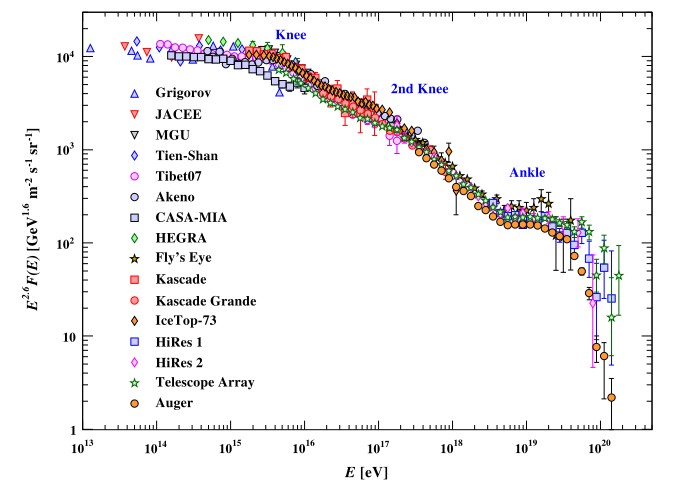
\includegraphics[scale = 0.5]{FIGURAS/ESPECTRO_RC.png}
	\caption{Espectro de flujo de rayos cósmicos a altas energías, multiplicado por $E^{2.6}$ para una mejor observación, en función de la energía \cite{MOLLERACH201885}.}
	\label{Espectro_CR}
\end{figure}

La figura \ref{Espectro_CR}, nos muestra el espectro de flujo de CR's a altas energías, este espectro sigue una ley de potencias de aproximadamente $d\phi /dE \propto E^{-\gamma}$ con un valor de $\gamma \simeq 3$, este espectro muestra algunas interesantes características.
\begin{itemize}
	\item Por encima de pocos cientos de GeV hasta pocos cientos de PeV, el espectro muestra un valor de $\gamma \simeq 2.7$.
	\item En la zona conocida como primera rodilla o ``kne" ($\sim 4 \mbox{PeV}$) el espectro cambia a $\gamma \simeq 3$.
	\item En la zona conocida como segunda rodilla o ``seoncd knee" ($\sim 0.1 \mbox{EeV}$) el espectro cambia a $\gamma \simeq 3.3$.
	\item En la zona concida como tobillo o ``ankle" ($\sim 5 \mbox{EeV}$), el espectro cambia nuevamente con $\gamma \simeq 2.6$.
\end{itemize}

Note que el flujo determinado por varios experimentos varía debido a las técnicas de detección y calibración de energía usado en los distintos experimentos. Además de que, para la detección de CR de altas energías se estudian las cascadas atomosféricas formadas por estos, ver sec. \ref{EAS}.